
\section{Design}
\label{sec:design}
This section presents the detailed design of \sysname.

\subsection{External Factor Sensing}
\label{subsec:external}
It is neither possible nor necessary to exhaust a complete list of influential factors on blood glucose concentration.
In \sysname, five major external factors are measured, including food, drug and insulin intake, as well as physical activities and sleep quality.

\fakeparagraph{Food Intake}
As food intake is a main source of carbohydrate, \sysname provides a food menu for users to keep track of their meals.
Based on the carbohydrate food list~\cite{bib:carblist}, meals are categorized into five types, including grains, vegetables, milk and egg, fruits and meats.
Users are asked to enter the food types and amounts of their meals, based on which \sysname calculates $U_C$, the carbohydrate of a meal.

\fakeparagraph{Drug Intake}
Oral diabetic drugs enhance the secretion of insulin into the blood and are usually used by type II diabetic patients.
In \sysname, a drug menu of 11 common oral diabetes is presented for users to input their drug intake based on \cite{bib:druglist}.
Users are required to select the drug name and record the dosage into \sysname.

\fakeparagraph{Insulin Injection}
Inulin injection is widely used for blood glucose control for type I and type II patients.
\sysname provides an insulin type list based on~\cite{bib:insulinlist} for users to record the usage and dosage of their insulin injection.
\sysname automatically transforms drug intake and insulin injection into the amount of acting insulin $U_I$ via bolus and basal rate information~\cite{bib:MAIHA14:Plis}.

\fakeparagraph{Physical Activity}
Daily activities \eg exercises consume the carbohydrate and affect blood glucose levels.
In \sysname, we adopt an efficient activity recognition scheme~\cite{bib:KDDEN11:Kwapisz} to automatically record six common physical activities (walking, running, going upstairs, going downstairs, sitting and standing) along with the corresponding durations.
\sysname then calculates the caloric expenditure based on the widely used calorie calculator~\cite{bib:HealthStatus, bib:CalorieCounter}.
\begin{equation}\label{eq:calorie_burn}
  Calorie Burn = (BMR/24)*MET*T,
\end{equation}
where BMR (Basal Methobolic Rate) is the amount of energy required to simply sit or lie quietly, and MET (Metabolic Equivalent) is the ratio of the work metabolic rate to the resting metabolic rate.
\sysname leverages the calorie expenditure $U_E$ as input for physiological feature extraction.

\fakeparagraph{Sleep Quality}
Sleep quality has a long-term influence on the blood glucose level~\cite{bib:DRCP15:Iwasaki}.
\sysname automatically measures sleep quality using smartphones as in~\cite{bib:UbiComp14:Gu}.
The output sleep quality score $U_S$ is then used for physiological feature extraction.

In summary, the five external factors are transformed into four categories of measurements including the carbohydrate of a meal ($U_C$), the amount of acting insulin ($U_I$), calorie expenditure ($U_E$) and sleep quality score ($U_S$), which are then used as input to extract important features for blood glucose level inference.

\subsection{Feature Engineering}
\label{subsec:features}
We extract features $X=\{X_P, X_T\}$ from external sensory data $U=\{U_C, U_I, U_E, U_S\}$ from both the physiological view ($X_P$, 10-dimension) and the temporal view ($X_T$, 51-dimension) to infer blood glucose levels, detailed as follows:

\subsubsection{Features from Physiological View $X_P$}
\label{subsubsec:physiological}
\begin{figure}[h]
  \centering
  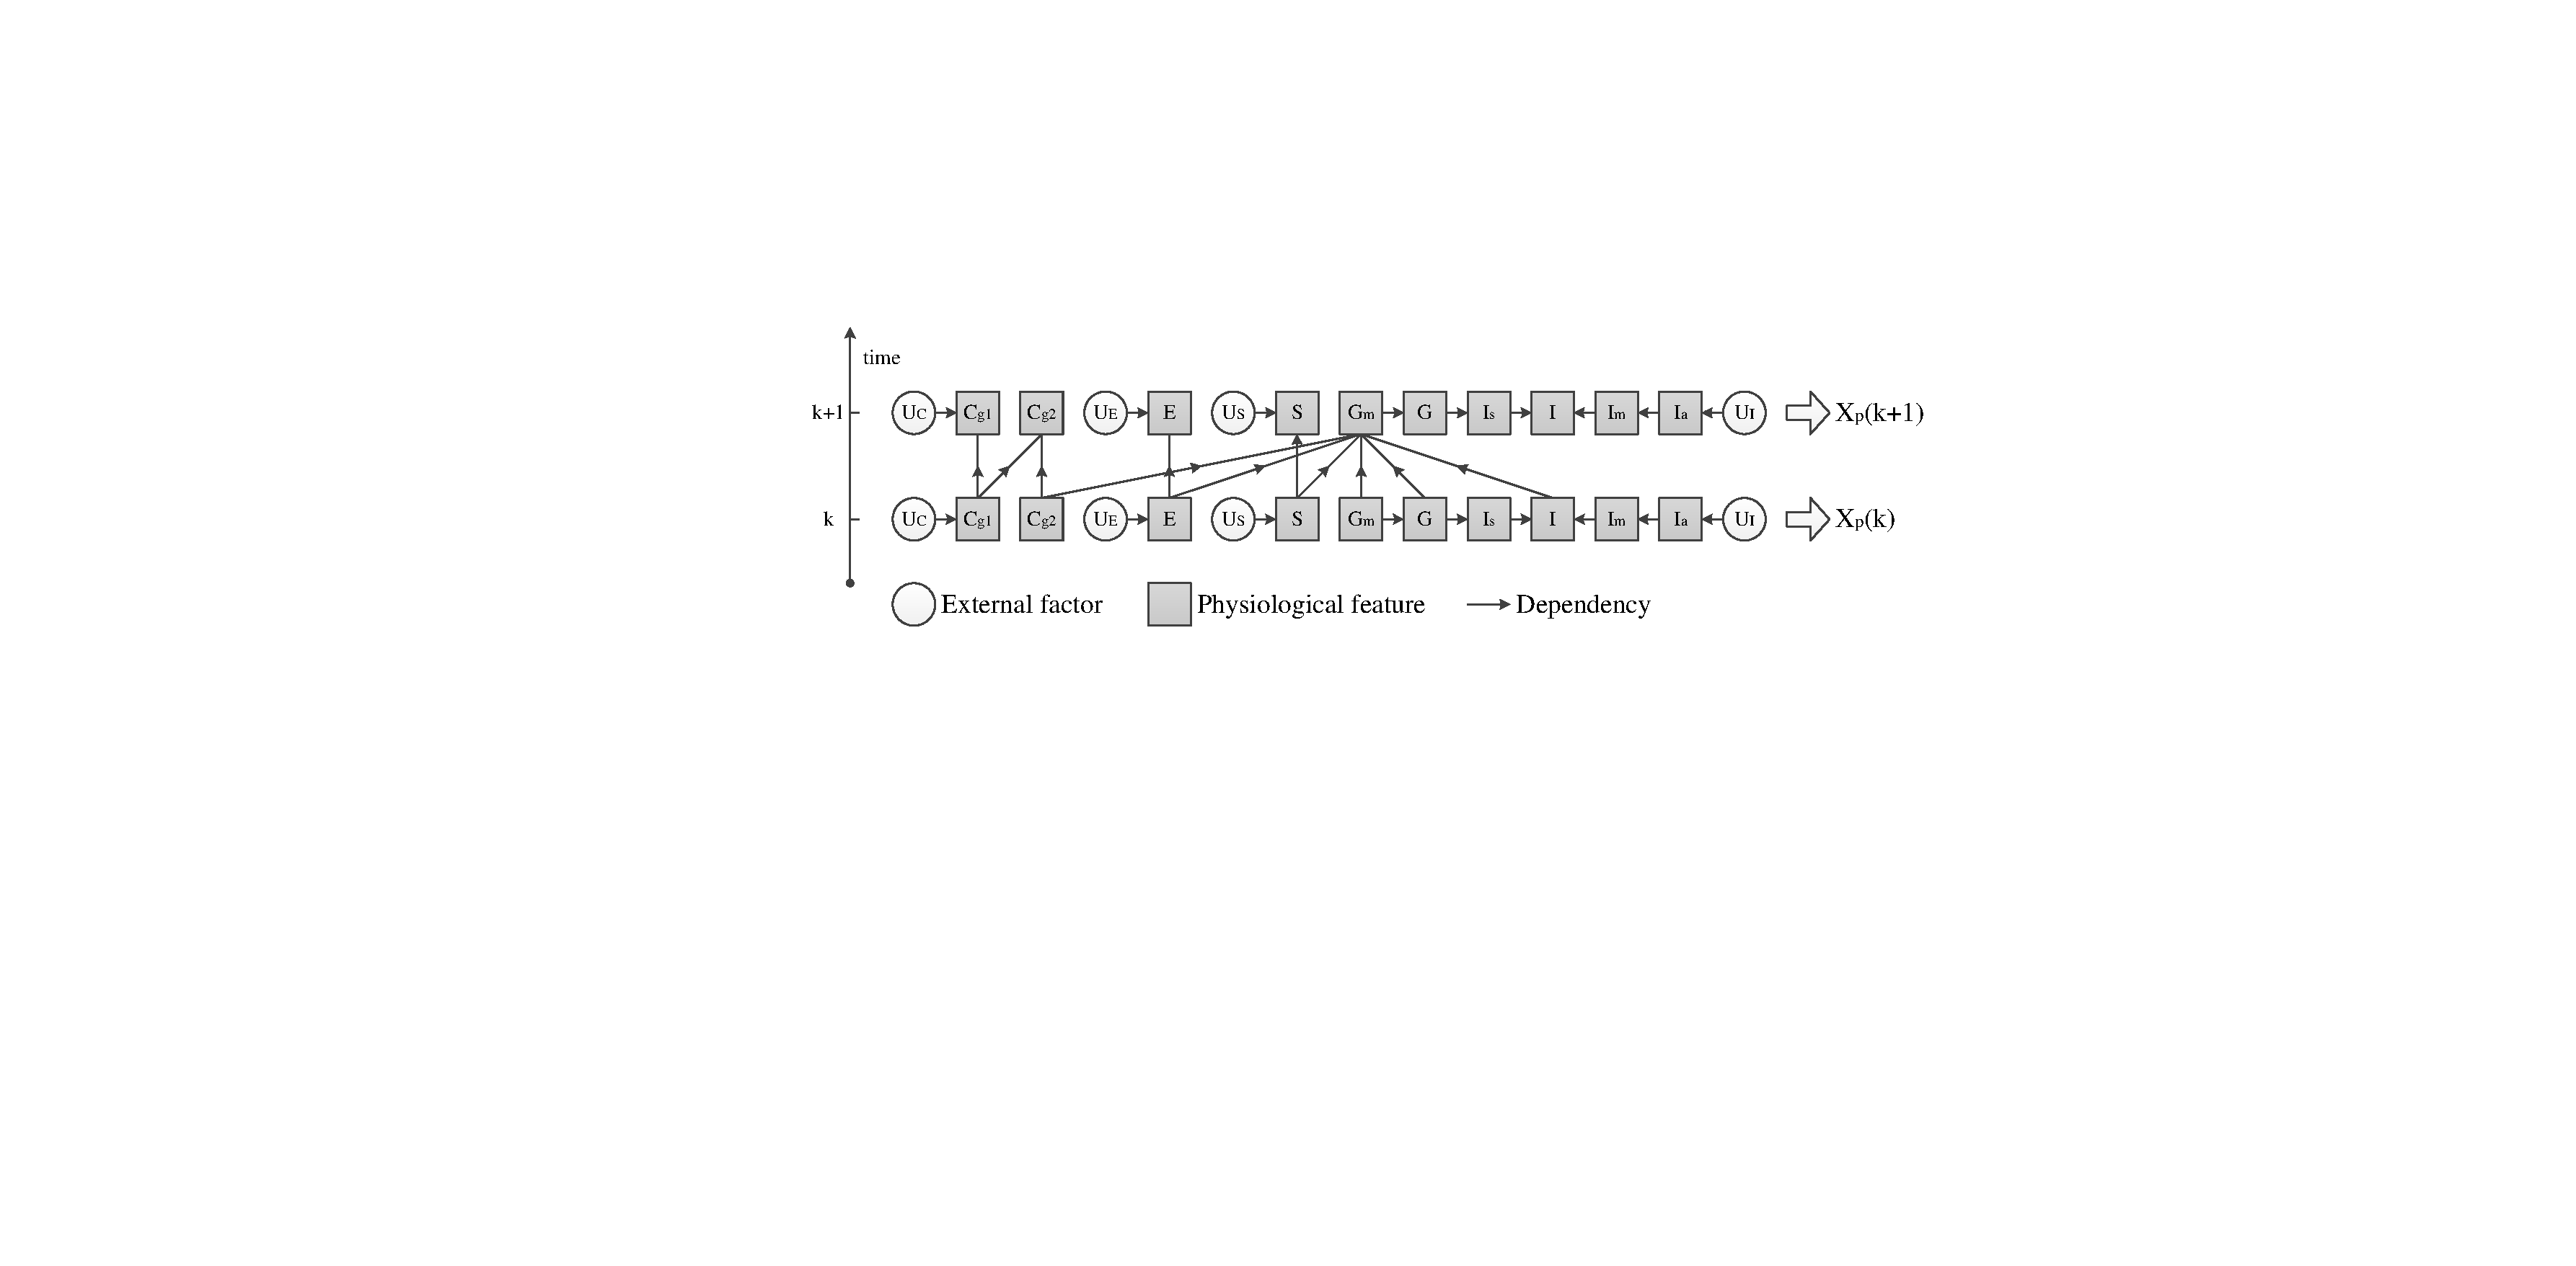
\includegraphics[width=0.9\columnwidth]{./img/Physiological_correlation2.pdf}
  \caption{An illustration of dependencies of physiological features $X_P=\{C_{g_1}, C_{g_2}, I_{a}, I_{m}, I_{s}, I, E, S,  G_{m}, G\}$ and of external factors $U=\{U_C, U_I, U_E, U_S\}$.}
  \label{fig:phymodel}
\end{figure}
\begin{table}[h]
  \centering
  \caption{Transition equations to calculate physiological features at time $k+1$ based on external factors measured at time $k+1$ and physiological features at time $k$~\cite{bib:duke2010intelligent, bib:MAIHA14:Plis}.}
  \label{tab:phyeq}
  \begin{tabular}{ll}
  \toprule
  \textbf{Dynamic Process} & \textbf{Transition Equations} \\
  \midrule
  Carbohydrate dynamics & $\begin{aligned}
                            C_{g_1}(k+1) &= C_{g_1}(k)-\alpha_{1}^c \times C_{g_1}(k)+U_{C}(k+1) \\
                            C_{g_2}(k+1) &= C_{g_2}(k)+\alpha_{1}^c \times C_{g_1}(k)-\alpha_{2}^c\times C_{g2}(k)
                          \end{aligned}$ \\
  \midrule
  Insulin dynamics & $\begin{aligned}
                            I_{a}(k+1) &= I_{a}(k)-\alpha_{f,r,m}^I\times I_{a}(k)+U_{I}(k+1) \\
                            I_{s}(k+1) &= I_{s}(k) \\
                            I_{m}(k+1) &= I_{m}(k)+\alpha_{f,r,m}^I\times I_{a}(k)+\alpha_{a}^I*I_{a}(k)-\alpha_c^I\times I_{m}(k) \\
                            I(k) &= I_{m}(k)\times S^I / (142 \times bm)
                          \end{aligned}$ \\
  \midrule
  Exercise dynamics & $E(k-k_0+1) = (k-k_0)\times E(k-k_0)+U_{E}(k-k_0+1)$ \\
  \midrule
  Sleep dynamics & $S(k-k_0+1) = (k-k_0)\times S(k-k_0)+U_{S}(k-k_0+1)$ \\
  \midrule
  Glucose dynamics & $\begin{aligned}
                            G_m(k+1) &= G_m(k)+\delta_{abs}+\delta_{egp}-\delta_{ind}-\delta_{dep}-\delta_{clr} \\
                            G(k+1) &= G_m(k+1)/(2.2\times bm)\\
                            \delta_{abs} &= \alpha_3^c\times\alpha_2^c\times C_{g_2}(k)\\
                            \delta_{egp} &= \alpha_2^{egp}\times \exp(-I(k)/\alpha_3^{egp})-\alpha_1^{egp}\times G(k)\\
                            \delta_{ind} &= \alpha_1^{ind}/\sqrt{G(k)} \\
                            \delta_{dep} &= \alpha_1^{dep}\times E(k)\times S(k)\times I(k)/(G(k)+\alpha_2^{dep}) \\
                            \delta_{clr} & =\alpha_1^{clr}\times (G(k)-\tau)
                          \end{aligned}$ \\
  \bottomrule
  \end{tabular}%
  \begin{tablenotes}
      \small
      \item
      \textbf{Note 1:} $S^I$ and $bm$ refer to the insulin sensitivity and body mass, respectively.
      \item
      \textbf{Note 2:} All $\alpha$'s in the transition equations are user-specific parameters that need to be tuned per-person.
      The default values of parameters in the physiological model are set based on \cite{bib:duke2010intelligent} and are further tuned for each person via 10-cross validations.
      \item
      \textbf{Note 3:} We set the time duration $k-k_0$ to 24 hours in exercise dynamics and 7 days in sleep dynamics, which optimize our experimental results and match with the conclusions of clinical results~\TODO{add citation}.
  \end{tablenotes}
\end{table}

Physiological features are essentially medical/biological indexes in a person's body, that describes the dynamics of glucose related variables~\cite{bib:duke2010intelligent, bib:MAIHA14:Plis}.
We extract physiological features based on the physiological model in~\cite{bib:duke2010intelligent}, which characterizes carbohydrate dynamics, insulin dynamics, exercise dynamics, and glucose dynamics.
We further include sleep dynamics, another important external factor that affects blood glucose levels~\cite{bib:DRCP15:Iwasaki}.
Specifically, the following physiological features are extracted to represent blood glucose relevant dynamics.
\begin{itemize}
  \item
  Features from \emph{carbohydrate dynamics}:
  carbohydrate consumption $C_{g_1}$ and carbohydrate digestion $C_{g_2}$.
  \item
  Features from \emph{insulin dynamics}:
  subcutaneous insulin absorption $I_{a}$, insulin secretion by pancreas $I_{s}$, insulin mass $I_{m}$ and active plasma insulin level $I$.
  \item
  Features from \emph{exercise dynamics}:
  long-term effect of exercises on insulin $E$.
  \item
  Features from \emph{sleep dynamics}:
  long-term effect of sleep quality on insulin $S$.
  \item
  Features from \emph{glucose dynamics}:
  glucose mass $G_m$ and glucose concentration $G$.
\end{itemize}
The features are inter-dependent and are also related to the external factors.
\figref{fig:phymodel} illustrates the dependencies among variables and \tabref{tab:phyeq} summarizes the transition equations to calculate the physiological features at time $k+1$ using external factor measurements at time $k+1$ and historical physiological features at time $k$.
The transition equations involve a set of parameters $\alpha$'s, e.g., the insulin sensitivity $S^I$ and the body mass $bm$.
Note that it is generally difficult to determine the parameters in the transition equations.
Therefore, the glucose concentration $G$ derived from the physiological model usually deviates from the actual blood glucose level.
It can be viewed as a ``nominal'' blood glucose indicator averaged out from the overall population.
Consequently, we exploit the glucose concentration $G$ derived from the physiological model as one dimension of the physiological features, which are fed into our \modelname framework to learn the complex, personalized dynamics of blood glucose.

%\emph{Carbohydrate dynamics}:
%Carbohydrate dynamics refer to the transitions of carbohydrate consumption $C_{g_1}$ and the carbohydrate digestion $C_{g_2}$.
%Equation~\ref{Eq:Cg1} and Equation~\ref{Eq:Cg2} show their transition equations respectively, where $U_{c}$ stands for the carbohydrate proportion of meals.
%\begin{equation}\label{Eq:Cg1}
%C_{g1}(t+1)=C_{g1}(t)-\alpha_{1}^c*C_{g1}(t)+U_{c}(t)
%\end{equation}
%
%\begin{equation}\label{Eq:Cg2}
%C_{g2}(t+1)=C_{g2}(t)+\alpha_{1}^c*C_{g1}(t)-\alpha_{2}^c*C_{g2}(t)
%\end{equation}

%\emph{Insulin dynamics}: Insulin dynamics indicates the transitions of subcutaneous insulin absorption $I_{a}$ (Equation~\ref{Eq:Is}),
%the insulin secretion by pancreas $I_{s}$ and  the insulin mass $I_{m}$ (Equation~\ref{Eq:Im}).
%The level of active plasma insulin $I$ (Equation~\ref{Eq:I}). $U_{I}$
%states for the amount of insulin injected or simulated by the diabetes drugs.
%
%$S^I$ and $bm$ refer to the insulin sensitive and body mass respectively.
%
%\begin{equation}\label{Eq:Is}
%I_{a}(t+1)=I_{a}(t)-\alpha_{f,r,m}^I*I_{a}(t)+U_{i}(t)
%\end{equation}
%
%
%\begin{equation}\label{Eq:Isec}
%    I_{s}(t+1)=
%   \begin{cases}
%    I_{s}(t)+min[\alpha_1^I(\alpha_2^I(G_t-G_0))+\alpha_3^I*G_0, \triangle I_{max}^{s}] &\mbox{Type II}\\
%    I_{s}(t)+0 &\mbox{Type I}
%   \end{cases}
%  \end{equation}
%
%\begin{equation}\label{Eq:Im}
%I_{m}(t+1)=I_{m}(t)+\alpha_{f,r,m}^I*I_{a}(t)+\alpha_{a}^I*I_{a}(t)-\alpha_c^I*I_{m}(t)
%\end{equation}
%
%
%\begin{equation}\label{Eq:I}
%I(t)=\frac{I_{m}(t)*S^I}{142*bm}
%\end{equation}

%\emph{Exercise dynamics}: Exercise dynamics $E$ denotes the exercise effect on insulin over the past time window.
%This long-term influence can be expressed by a cumulative moving average \cite{bib:lowry1992multivariate, bib:cma} as Equation~\ref{Eq:E} in the physiological model.
%
%\begin{equation}\label{Eq:E}
%E(t-t_0+1)=(t-t_0)*E(t-t_0)+U_{e}(t-t_0)
%\end{equation}

%where $t$ and $t_0$ are the current and beginning time point in the past time window. In \sysname,
%the window size of exercise is set to 24 hours, which optimizes the experimental results and matches the conclusion
%of clinical studies.
%
%\emph{Sleep dynamics}: Sleep dynamics $S$ represents the sleeping quality effect on insulin. In physiological model, sleeping
%effect also has a long-term influence on the insulin as the exercise effects. Specifically, it maintains a constant effect on
%blood glucose for each day. Equation~\ref{Eq:S} shows its transition equation.
%
%\begin{equation}\label{Eq:S}
%S(t-t_0+1)=(t-t_0)*S(t-t_0)+U_{s}(t-t_0)
%\end{equation},
%
%where $t$ and $t_0$ are the current and beginning time point in the past time window.
%In \sysname, the window size of sleep lasts for 7 days, which optimizes the experimental results and matches the conclusion
%of clinical studies.


%\emph{Blood glucose dynamics}: Blood glucose dynamic points to the fluctuation of glucose mass $G_m$  in Equation~\ref{Eq:Gm},
%and glucose concentration $G(t)$ in Equation~\ref{Eq:G}.
%\begin{equation}\label{Eq:Gm}
%G_m(t+1)=G_m(t)+\delta_{abs}+\delta_{egp}-\delta_{ind}-\delta_{dep}-\delta_{clr}
%\end{equation}
%\begin{equation}\label{Eq:G}
%G(t)=G_m(t)/(2.2*bm)
%\end{equation}
%
%Specifically, $\delta_{abs}$ in Equation~\ref{Eq:abs} refers to the impact results of carbohydrate absorption, and
%$\delta_{egp}$ in Equation~\ref{Eq:egp} indicates to the hepatic glucose production from
%the liver. These two factors improve the blood glucose concentration of body.
%\begin{equation}\label{Eq:abs}
%  \delta_{abs}=\alpha_3^c*\alpha_2^c*C_{g2}
%\end{equation}
%
%\begin{equation}\label{Eq:egp}
%  \delta_{egp}=\alpha_2^{egp}*exp(-I(t)/\alpha_3^{egp})-\alpha_1^{egp}*G(t)
%\end{equation}
%
%$\delta_{ind}$ (Equation~\ref{Eq:ind}) describes results of insulin independent uptake, which is consumed by the central nervous
%system and the red blood cells.
%$\delta_{dep}$ (Equation~\ref{Eq:dep}) indicates the impact results of insulin dependent uptake. It reflects the effects
%of insulin promoting muscle cells and fat cells to absorb glucose, which combines the influence of sleeping and exercise factors.
%$\delta_{clr}$ (Equation~\ref{Eq:clr}) stands for the influence of renal clearance on blood glucose. Once blood glucose
%concentrations exceeds the renal clearance threshold $\tau$, the kidneys begin to remove excess glucose from the blood.
%The three factors decrease the blood glucose level.
%
%\begin{equation}\label{Eq:ind}
%  \delta_{ind}=\alpha_1^{ind}/\sqrt{G(t)}
%\end{equation}
%
%\begin{equation}\label{Eq:dep}
%  \delta_{dep}=\alpha_1^{dep}* E(t)*S(t)*I(t)/(G(t)+\alpha_2^{dep})
%\end{equation}
%
%\begin{equation}\label{Eq:clr}
%  \delta_{clr}=\alpha_1^{clr}*(G(t)-\tau)
%\end{equation}
%
%with an extension of sleeping fact according to its physiological impact discussed in.


%\paragraph{Temporal Graph of Physiological Model}
%The physiological model of \sysname describes the physiological factors from five aspects:

%Given the hidden physiological vectors $X_{t}=\{C_{g1}(t), C_{g2}(t),\\ I_{s}(t),I_{m}(t), I_{t}, G_{m}(t), G(t), E(t)\}$, where the elements of this vector represent
%the hidden physiological factors at time point $t$, and the observable input vector $U_{t}=\{U_{c}(t), U_{e}(t), U_{s}(t), U_{i}(t)\}$ , in which $U_{c}$ stands for the
%carbohydrate proportion of meals, $U_{e}$ indicates the calories cost by exercise,  $U_{s}$ is the sleep score and $U_{i}$ states for the amount of insulin injected or simulated
%by the diabetes drugs  at time point $t$. In particular, the sleep quality $U(s)$ is a constant during a whole day.
%The station transition functions can be represented as $X_{t+1}=f(X_t, U_t)$, and its corresponding
%temporal transition graph is shown as \figref{fig:phymodel}.  %\tabref{phy_tab} details the transformation functions of the carbohydrate $C_{g1}$ and $C_{g2}$, and insulin
%As \figref{fig:phymodel} shown, the equations of $C_{g1}$ (Equation~\ref{Eq:Cg1}) and $C_{g2}$ (Equation~\ref{Eq:Cg2}) indicating the temporal transitions of carbohydrate consumption and the carbohydrate digestion respectively.

%Positive factors of physiological model indicate the carbohydrate absorption and the hepatic glucose production, which will increase the blood glucose level.
%Negative factors of  physiological model describe the insulin independent uptake, insulin dependent uptake and the renal clearance. We will detail these factors as follows:

%
%In \sysname, we use smartphone to collect the external factors $U_t=\{U_c(t),U_e(t),U_s(t), U_i(t)\}$, and
%apply the physiological model to generate real-time observed vector
%$X_{t}=\{C_{g1}(t), C_{g2}(t),I_{s}(t),I_{m}(t), I_{a}(t), I(t),\\
% E(t), S(t),  G_{m}(t), G(t)\}$ for every blood glucose sample at the corresponding time $t$.
%The hidden physiological factors at $t+1$ can be calculated by
%$X_{t+1}=f(X_t, U_t)$, where $f$ is the station transition functions.
%\sysname computes $X$ at each time step and treats it as 10-dimensional
%features.

\subsubsection{Features from Temporal View $X_T$}
As blood glucose level naturally varies over time, we extract two temporal features for blood glucose level inference.
\begin{itemize}
  \item
  History blood glucose concentration $X_{T_1}$ at time $k$:
  Since people usually tend to lead a regular lifestyle, \eg having meals in the morning, at noon and in the evening and sleep at night, the blood glucose concentration also exhibits rough daily cycles.
  \figref{fig:XXX} plots the daily blood glucose traces of a volunteer for six successive days measured by a CGM device.
  \TODO{explain the figure, \eg always peak at XXX, XXX, XXX time, due to \eg meals, and...}
  This motivates us to adopt the historical blood glucose concentrations at time stamp $k$ (averaged over $D$ days) as one temporal feature to infer the blood glucose level at time $k$.
  In \sysname, we set $D=5$ and infer blood glucose level at a time resolution of 3min, which is in accordance with the time resolution of commercial CGM devices~\cite{bib:CGM_wave}.
  \item
  Most recent physiological features $X_{T_2}$:
  As shown in the physiological models, the current blood glucose concentration is relevant to the recent blood glucose concentration and physiological features.
  However, in the physiological features $X_P$, only the physiological features at the last time stamp are considered.
  To account for more short-term temporal dependencies, we propose to include the $l$ most recent physiological features $X_{T_2}(k) = \{X_P(k), X_P(k-1), \ldots, X_P(k-l+1)\}$, where $l=5$ in our implementation.
  That is, instead of considering the physiological features in the last 3min, we infer the current blood glucose level leveraging features in the last 15min.
\end{itemize}
In summary, we extract a 51-dimension ($1+10\times 5$) temporal feature vector $X_T$ for blood glucose level inference.
%Considering the physiological features may generate the temporal delay effects on the blood glucose, \sysname also takes the physiological factor vectors in the past 15 minutes as recent physiological features to measure their impacts on the current blood glucose concentration.

%\paragraph{Historical Blood glucose trend: $F_{t1}$}
%Since the trend of blood glucose of a single person hardly occurs significant alteration within a short period, \sysname calculates the historical blood glucose trend $G_{Trend}$ by average the true blood glucose concentrations at each corresponding time stamp $t$ over recent $D$ days in the past by Equation~\ref{Eq:his_trend}.
%
%\begin{equation}\label{Eq:his_trend}
%  G_{Trend}=\frac{1}{D}\sum_{d=1}^{D}G(f_t(d)),  t=1,2,...,N
%\end{equation}
%
%where $N=480$ refers to the number of time stamps in a day, and $D$ reflects the days of measurement.
%$G(f_t(d))$ indicates the true blood glucose value measured by the CGM at the time stamp $t$ of the $d$th day.
%In \sysname, we select $D=5$ based on the optimal experimental results

%\sysname treats it as a temporal feature to reflect the historical blood glucose trend over the same period.

%\TODO{Is it temporal feature?}
%\paragraph{Blood glucose value with similar physiological features: $F_{t2}$}
%As the blood glucose concentrate is determined by the factors of carbohydrate, insulin, exercise intensity and sleep quality, the similar blood glucose values should maintain similar values of these physiological factors.
%Accordingly, \sysname applies the k-Nearest Neighbors algorithm \cite{bib:KNN} to search for 5 blood glucose values with the most similar physiological features, and average them as one dimensional feature.

%\paragraph{Recent physiological features: $F_{t3}$}
%Considering the physiological features may generate the temporal delay effects on the blood glucose, \sysname also takes the physiological factor vectors in the past 15 minutes as recent physiological features to measure their impacts on the current blood glucose concentration.
%
%\sysname takes the physiological-temporal features as input, and predict the blood glucose level by \modelname.


\subsection{Blood Glucose Level Inference}
Given the features extracted based on the physiological process, it seems plausible to perform any classification algorithm for blood glucose level inference.
Nonetheless, this plug-and-play approach will neglect important information from (1) dynamics of the process, and (2) inter-user similarity among the same group of participants.
Traditionally, various sequential classification methods [], \eg hidden Markov model (HMM) and recurrent neural networks (RNN), are used to capture the temporal correlation of the input feature.
The inter process correlations are often times incorporated with the so-called multi-task learning approaches [], which learns processes (or tasks) in parallel to improve classification or to reduce the data sample requirement.

In this paper, a novel machine learning paradigm, namely Multi-division deep-dynamic RNN (\modelname), is proposed.
To include the the aforementioned information sources in an unified framework, we develop two key ideas that extend the classical RNN. Firstly, the single hidden layer in RNN is replaced with several deep stacked layers.
The deep structure in the new model is able to describe complex, multi-scale dynamics that would otherwise be ignored (or averaged out) by prior ``shallow'' models.
Secondly, the correlations among users, being quite significant within user groups (divisions), are encoded by group-shared input layer and common hidden layers, whereas the distinct characteristics of individual users are modeled with different output layers for personalized prediction.
Within a larger scope of machine learning, the proposed \modelname aims to leverage recent advancement of deep learning and multi-task learning, to model group-interacted time series data having complex temporal dynamics.
It can be viewed as both a deep extension of RNN, and an intermediate between single-task learning and multi-task learning, hence the name.
Although we develop \modelname for the specific use case of \sysname, it is worth pointing out that it can be readily applied to many other applications dealing with grouped dynamic data. 
The overall configuration of the proposed model is summarized in \figref{fig:rnn}.
Detailed construction of each component is given in the sequel.

\begin{figure}[h]
  \centering
  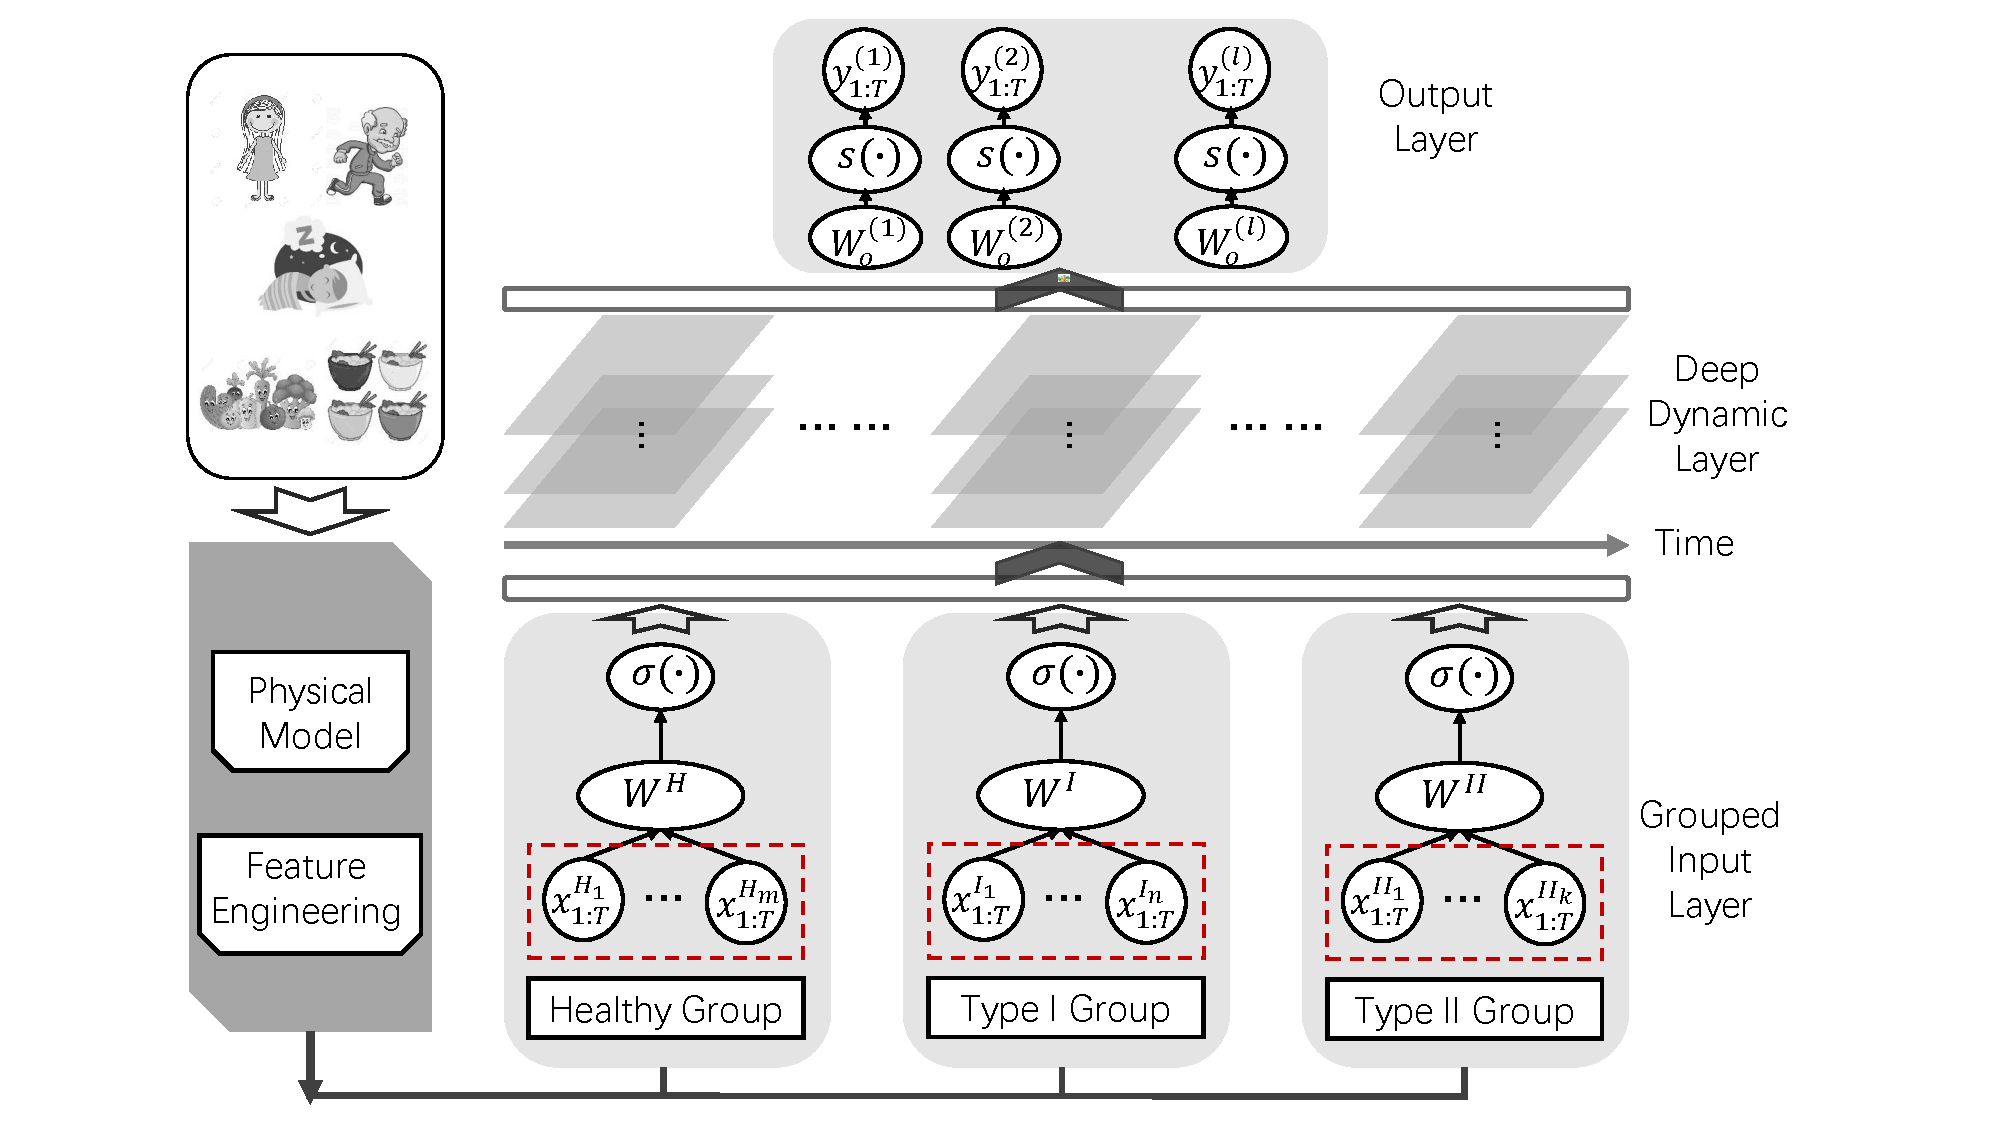
\includegraphics[width=0.9\columnwidth]{./img/pics_RNN2.pdf}
  \caption{Illustration of \modelname structure.}
  \label{fig:rnn}
\end{figure}

\subsubsection{Model construction by layers}
The inputs of the \modelname model are the features extracted following the discussion in the previous section.
The labeled data sequences for user number $j$ at time $i$ are denoted by $(x_i^{j},y_i^{j})$.
We also adopt an index set convention, that $(x_A^{B},y_A^B)$ represents the data set $\left\{(x_i^{j},y_i^{j}) | i \in A, j\in B\right\}$ given index sets $A$ and $B$.

\fakeparagraph{Grouped Input Layer}
In the context of blood glucose prediction, available inputs are naturally divided into three groups according to the health condition of the participant from whom the data was generated.
Notation-wise, we utilize $H$, $I$ and $II$ to indicate the the group of healthy user, user with type I diabetes and those having type II diabetes, respectively.
Since the extracted features are essentially physiological indexes and temporally correlated variables, they must go though different transformations to represent useful information of three distinct groups.
This consideration motivate the design of the input layer (bottom of \figref{fig:rnn}) - it is divided into three units that performs different linear and non-linear transformation according to user groups.
For instance, a data sample $x_t^{I_j}$, generated at time $t$ from the $j^{th}$ user of type I, undergoes the following processing:
\begin{align}
\tilde{x}_t^{I_j} = \sigma \left( W^Ix_t^{I_j} \right)
\end{align}
where $W^I$ is the coefficients of the affine transformation \footnote{We assume that the interception is included in $W$. This can be done by simply adding a feature of all $1$s.}, $\sigma$ is the activation function, and $\tilde{x}_t^{I_j}$ is the output of the input layer for that data sample.
Similar operations are conducted for data samples from group $H$ and $II$, but with different transformation coefficients.
Intuitively, the shared transformation within groups would improve the learning of parameters (vs. single task learning), as information from all data in a homogeneous group is used.
Also, the transformation can be stacked into several (say $P$) layers, for better information representation.

\fakeparagraph{Deep Dynamic Layer}
A common hidden layer is designated to capture the dynamics of the blood glucose evolution process.
The underlying assumption is that, the biological and chemical reactions governing blood glucose variation are similar for all people, despite of grouped behaviors in the representation of physiological indexes (input layer), or individual characteristics in exhibited glucose level.
This assumption could be justified by a series of medical research[][].
Moreover, since all users share the same hidden layer, all collected data samples are eventually helping the estimation of its parameters.
The availability of rich information for the hidden layer makes the learning of a deep structure possible.
In \sysname, a number of Long Short Term Memory (LSTM) networks are stacked together (middle of \figref{fig:rnn}), to increase the overall model flexibility.
It has been justified in both theory and practice that stacked LSTMs are able to capture dynamics occurring at different time scales, which in the current application would enable the modeling of both slow and rapid biological/chemical reactions.
Although a wide variety of LSTM configuration exist in literature, in this work we adopt the one recently proposed by [], which combines the forget/input gate and merges cell/hidden state for simplicity and better generalization performance.
Mathematically, given the output from the grouped input layer, the deep dynamic layer performs
\begin{equation}
\begin{aligned}
&z^d_t = \sigma^d\left( W^d_z [h_{t-1}^d,h_t^{d-1}] \right) \\
&r^d_t = \sigma^d\left( W^d_r [h_{t-1}^d,h_t^{d-1}] \right) \\
&\tilde{h}_t^d = tanh\left( W^d_h [r_t^d*h_{t-1}^d,h_t^{d-1}] \right) \\
&h^d_t = (1-z_t^d)*h_{t-1}^d + z_t^d*\tilde{h}_t^d
\end{aligned}
\end{equation}
for hidden layer numbered $d = 1,2,\cdots,D$. At the first dynamic layer with $d=1$, the input $h_t^{d-1}$ is set to be the output from the grouped input layer, and the output of the last dynamic layer, $h^D_t$, will be used as the input of the last component of \modelname.

\fakeparagraph{Personalized Output Layer}
Finally, each user is assigned a personalized output layer, parameterized by $W_o^j, j=1,\cdots,l$, which performs a single linear and softmax transformation on the results of the deep dynamic layer.
The particular configuration of the output layer compensates for the individual characteristics in the exhibited blood glucose (\ie measured blood glucose level).
Because only data generated by a specific participant $j$ will have an effect on the its parameters $W_o^j$, the personalized output layer is set to have a ``shallow structure'', \ie it only performs the transformation once.
More specifically, given $h^D_t$ from user $j$, it computes
\begin{equation}
\hat{y}_t^j = \text{softmax} \left( W_o^j h^D_t \right)
\end{equation}

\subsubsection{Cost Sensitive Learning and Hyperparamter (Model) Selection}
Similar to other deep neural network learning, \modelname is trained by minimizing the sum of losses over all the time steps.
The definition of the loss function has much bearing on the generalization performance of the method.
In particular for the current application, simply minimizing a general error rate seems inappropriate, because the costs of different types of misclassifiction errors can differ a lot.
For example, missing the detection of high blood glucose (type I or II) is more costly than misclassifying normal condition to an alarm for high glucose.
Moreover, in the collected data set from real people, the training data is inherently imbalanced - the available samples labeled Level 1 and Level 4 are much fewer (only 7\%) compared to samples in the other categories (Level 2 and Level 3).

The above concerns motivate the cost sensitive learning of \modelname.
Instead of directly minimizing a surrogate of error rate, we propose to optimize over a weighted version of classification losses[].
More specifically, the following total loss function is considered:
\begin{equation}
L = \sum_{t} \sum_{y_t \in \mathcal{Y}} l(y_t,\hat{y}_t)C_{y_t}
\end{equation}
where $\mathcal{Y}$ is the label set, and $\hat{y}_t$s are prediction output from \modelname.
Our implementation uses cross entropy for $l(y_t,\hat{y}_t)$, but generally the ``base'' lost function $l(y_t,\hat{y}_t)$ can be any surrogate of the error function.
The additional coefficient $C_{y_t}$ weights the misclassification error for category $y_t$.
In the current application, $\mathcal{Y} = \{1,2,3,4\}$, associated with four coefficients $C_1$ to $C_4$.
Those cost weighting coefficients are treated as hyperparameters of the proposed model, but in other applications of \modelname, they can also be determined with prior knowledge about the misclassification cost and the class imbalance.

With the technique of back-propagating, computing the gradient of \modelname is not so different from the gradient calculation of classical RNN.
In this work, we accomplish those computation using Tensorflow [], and proceed to learn \modelname model by stochastic gradient descent for overall loss minimization.

Last but not least, the construction of the \modelname model involves choosing 15 hyperparameters, \eg cost coefficients $C_{y}$, depth $D$ of the stacked dynamic layer, learning rate, number of hidden unit in the input layer, \etc
Direct application of cross validation (CV) for hyperparameter tuning, even with the help of parallel computing, seems intractable as the number of required CVs scales exponentially to the number of hyperparameters.
In this regards, we adopt Bayesian optimization (BO), a recent tool developed for blackbox function optimization with limited evaluations.
The decision variables of BO are those hyperparameters, and the objective is the F-score of the precision and recall on some testing data set.
Note that BO has been used recently for the hyperparameter (model) selection of many deep learning paradigms [][].



